\documentclass[twocolumn,english]{IEEEtran}
\usepackage[T1]{fontenc}
\usepackage{babel}
\usepackage{amsthm}
\usepackage{amsmath}
\usepackage{graphicx}
\usepackage[unicode=true,
 bookmarks=true,bookmarksnumbered=true,bookmarksopen=true,bookmarksopenlevel=1,
 breaklinks=false,pdfborder={0 0 0},backref=false,colorlinks=false]
 {hyperref}
\usepackage{bm}
\usepackage{amsmath}
\usepackage{amssymb}
\usepackage{natbib}
\usepackage{array}
\usepackage{calc}
\newcommand{\vb}[1]{\mathbf{#1}}		%Bold vector
\newcolumntype{W}{>{\centering\arraybackslash}m{25mm}}
\newcolumntype{L}{>{\centering\arraybackslash}m{15mm}}
\usepackage{booktabs}

%%%%%%%%%%%%%%%%%%%%%%%%%%%%%%%%%%%%%%%%%%%%%%%%%%%%%%%%%%%%%%%%%%%%%%%%%%%%%%% Variables
\newcommand{\thetitle}{Project 4: Survey and Analysis}
\newcommand{\theauthors}{Zack Garza}
\newcommand{\theclass}{Math 142: Elementary Statistics}
%%%%%%%%%%%%%%%%%%%%%%%%%%%%%%%%%%%%%%%%%%%%%%%%%%%%%%%%%%%%%%%%%%%%%%%%%%%%%%%%%%%%%%%%%%

\hypersetup{
 pdftitle=  {\thetitle},
 pdfauthor= {\theauthors},
 pdfpagelayout=OneColumn, pdfnewwindow=true, pdfstartview=XYZ, plainpages=false}

\makeatletter


%%%%%%%%%%%%%%%%%%%%%%%%%%%%%% Textclass specific LaTeX commands.
 % protect \markboth against an old bug reintroduced in babel >= 3.8g
 \let\oldforeign@language\foreign@language
 \DeclareRobustCommand{\foreign@language}[1]{%
   \lowercase{\oldforeign@language{#1}}}
\theoremstyle{plain}
\newtheorem{thm}{\protect\theoremname}
\theoremstyle{plain}
\newtheorem{lem}[thm]{\protect\lemmaname}

%%%%%%%%%%%%%%%%%%%%%%%%%%%%%% User specified LaTeX commands.
% for subfigures/subtables
\ifCLASSOPTIONcompsoc
\usepackage[caption=false,font=normalsize,labelfont=sf,textfont=sf]{subfig}
\else
\usepackage[caption=false,font=footnotesize]{subfig}
\fi

\makeatother
\providecommand{\lemmaname}{Lemma}
\providecommand{\theoremname}{Theorem}
\setcounter{topnumber}{2}
\setcounter{bottomnumber}{2}
\setcounter{totalnumber}{4}
\renewcommand{\topfraction}{0.85}
\renewcommand{\bottomfraction}{0.85}
\renewcommand{\textfraction}{0.15}
\renewcommand{\floatpagefraction}{0.7}
\usepackage{float}
\onecolumn

\usepackage{Sweave}
\begin{document}

\title{\thetitle}
\author{\theauthors}
\IEEEspecialpapernotice
{\theclass \\ Effective Date of Report: \today }
\markboth{\thetitle}{\theauthors}
\maketitle
\tableofcontents


\hrulefill

\section{Theme}
\IEEEPARstart{T}he theme of this project was to take samples from publicly available data sets, specifically those related to education. The California Department of Education amalgamates statistics on the several thousand schools in the state, and makes them freely available online. Thus, in this report, my goal is to explore these data sets, to examine the information within, and to hopefully glean useful information about the state of the education system in California.

\newpage




\section{Description}
Several data sets were downloaded and queried for information. The first was a yearly report from 2012 on the number of students eligible for enrollment in free or reduced priced meal plans (FRPM). The data examined was the proportion of students K-12 eligible for these programs, and how this related to what school or county they were in.

The second data set was a statewide report of annual STAR test results, an mandatory exam unique to California, given in 2012 to K-12 students statewide. The data queried from this set involved the schoolwide means for the 2012 exams, which were scored on a scale of 150-600. These two sets provided the quantitative portion of this project.

The qualitative portion was drawn from a separate lookup table that listed school and county codes, as well as tallys for the parental education levels for children attending each school.

\subsection{Population and Sample}

The population for this study consists of K-12 students in California, while the samples will be groups of schools and how they perform as a whole. The purpose of this investigation is to discover whether the aforementioned statistics remain constant across the state, or vary based on location.

\subsection{Sampling Technique}
To begin with, both data sets were downloaded, and extraneous results (such as state-wide or county-wide tallies) were filtered out. 
The remaining data described 8562 schools in 1575 disricts, distributed among 58 counties in California. 

The average number of schools per county was around 150, meaning that there was over a 97\% chance that selecting any county would result in a sample size greater than 30. 
Thus, this method provided a very high probability of fulfilling the requirement of $n \geq 30$ required for many of the following statistical analyses.

To select two independent populations, two counties were selected at random.

From the two chosen counties, simple random samples of 50 schools were taken without replacement from all of the districts and schools within that county.

From this data, a list of unique school codes were generated. 
This allowed cross-referencing the primary data sets.


\subsection{Survey Questions}
The schools codes were matched up with the STAR scores in the first data set, and the reduced/free lunch statistics in the second data set. 
This essentially amounted to "querying" the two samples in the following ways:

\begin{itemize}
		\item \textbf{Quantitative}:

				What was the average STAR score among K-12 students at this school?

				What proportion of this school's student population qualifies for free or reduced lunch?
		\item \textbf{Qualitative}:

				What were the students' parental education levels at this school?
\end{itemize}


\section{Data and Analysis}

\subsection{Free and Reduced Price Lunch}
\begin{figure}[H]
		\begin{centering}
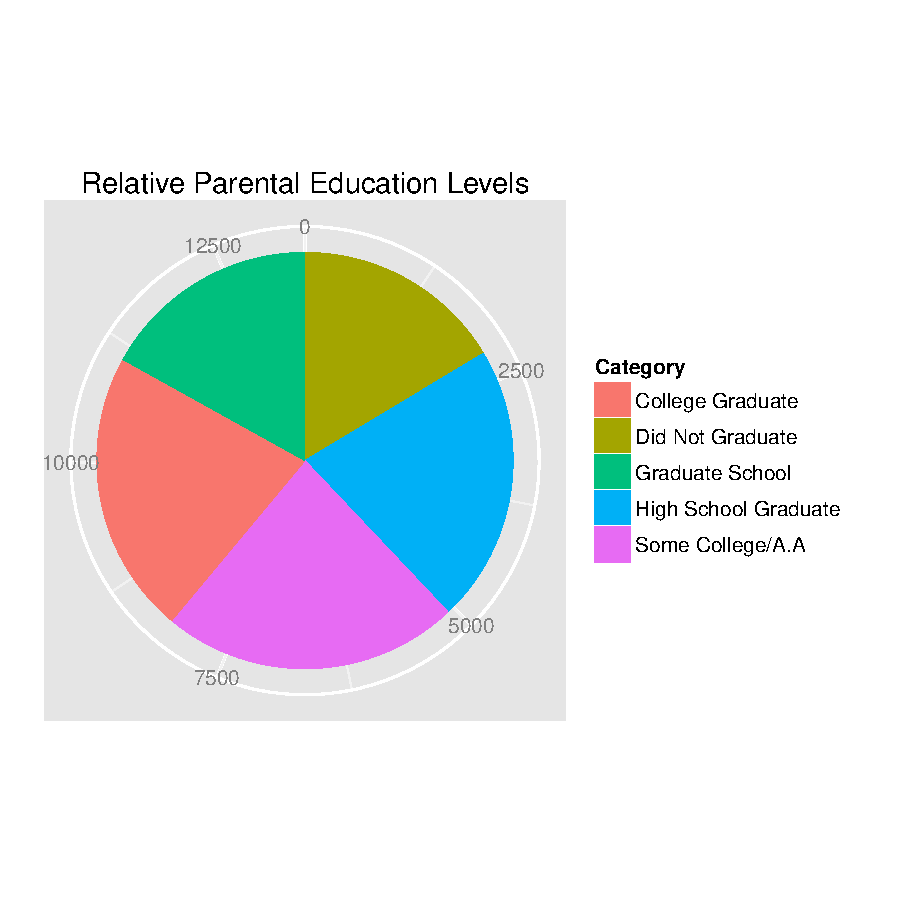
\includegraphics{proj3-pie_1}
		\caption{Levels of Parental Education Across Both Counties}
		\label{fig:pie_education}
		\end{centering}
\end{figure}


\begin{figure}[H]
		\begin{centering}
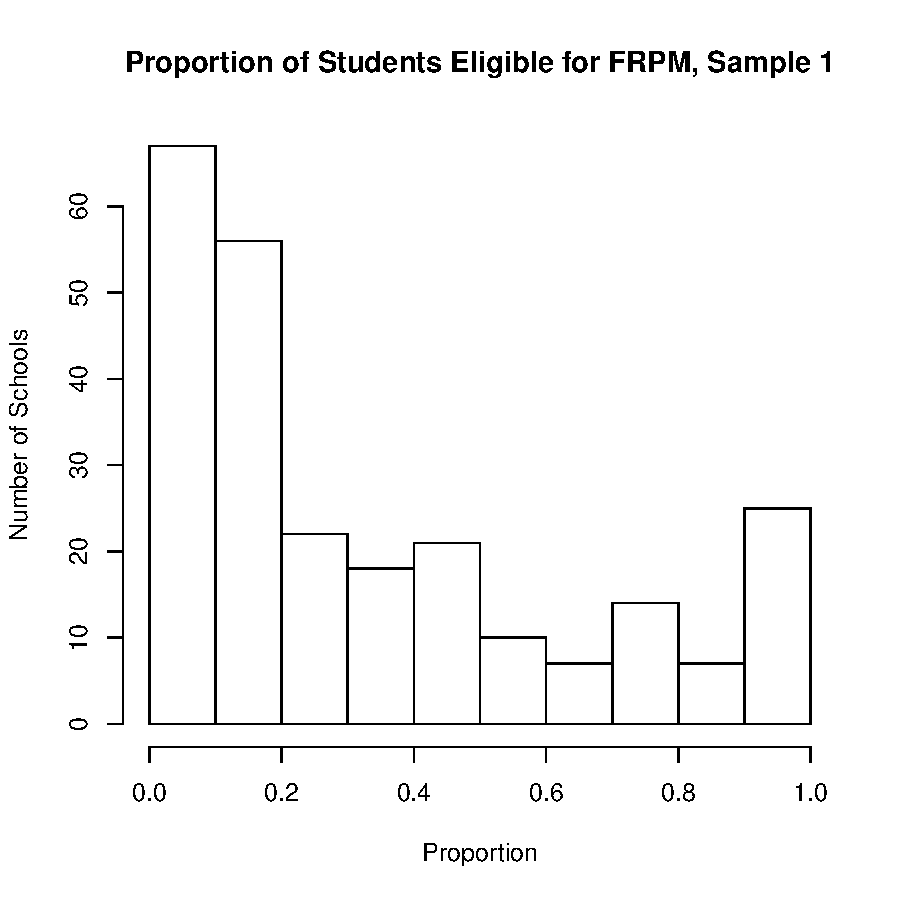
\includegraphics{proj3-fig_lunch_props2}
		\caption{Proportion of children attending each school that are eligible for free or reduced priced lunches, taken from the schools in sample one.}
		\label{fig:Lunch_Hist_Two}
		\end{centering}
\end{figure}


\begin{figure}[H]
		\begin{centering}
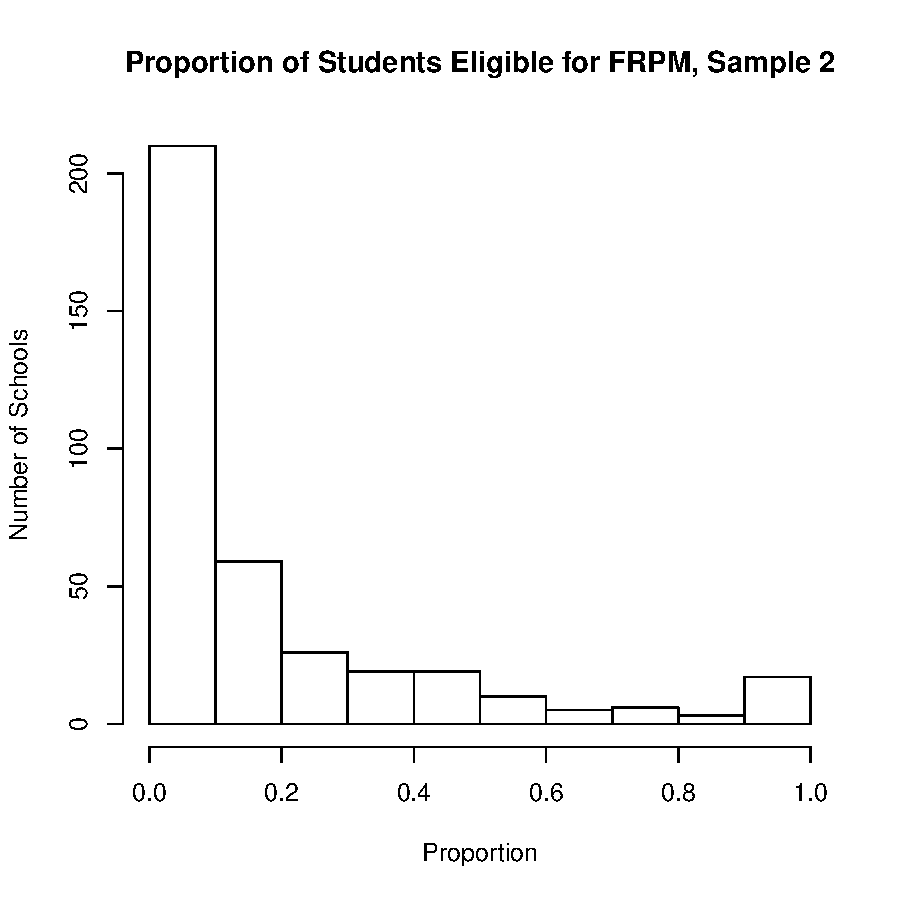
\includegraphics{proj3-fig_lunch_props1}
		\caption{Frequency polygon showing proportions of student populations eligible for free or reduced priced lunch in sample two.}
		\label{fig:Lunch_Hist_One}
		\end{centering}
\end{figure}


\subsection{State of California K-12 STAR Test Results}

\begin{figure}[H]
		\begin{centering}
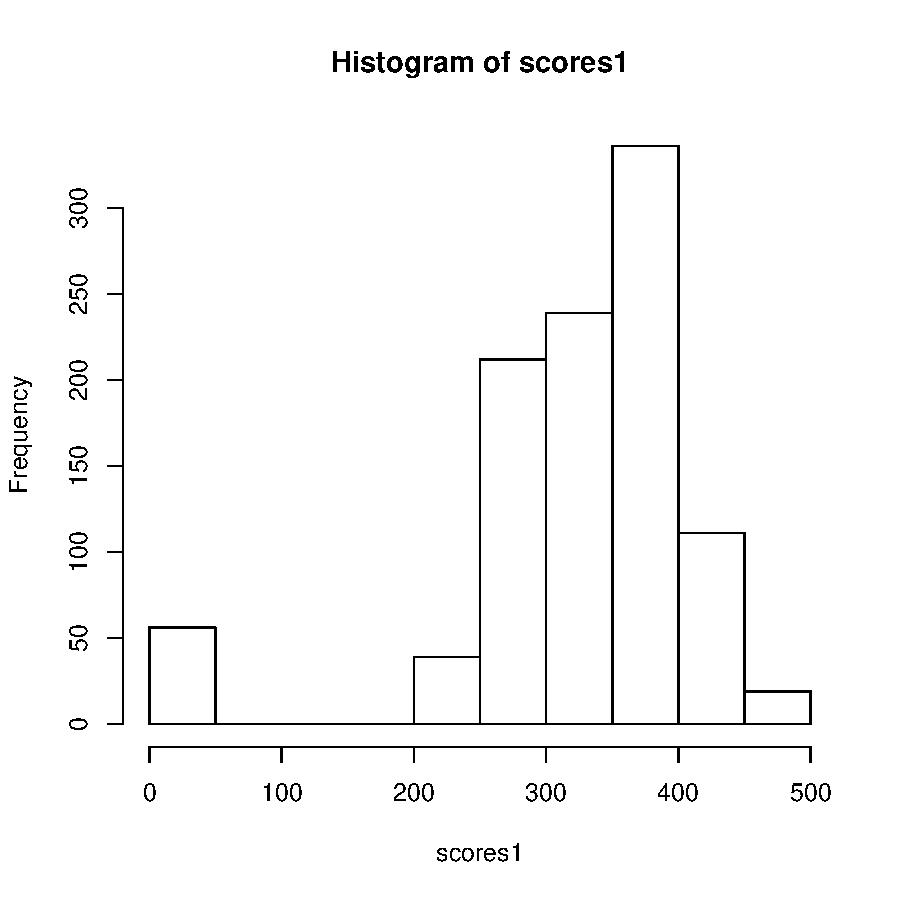
\includegraphics{proj3-fig_scores1}
		\caption{Sample One Score Distribution}
		\label{fig:Scores_Hist_One}
		\end{centering}
\end{figure}


\begin{figure}[H]
\begin{centering}
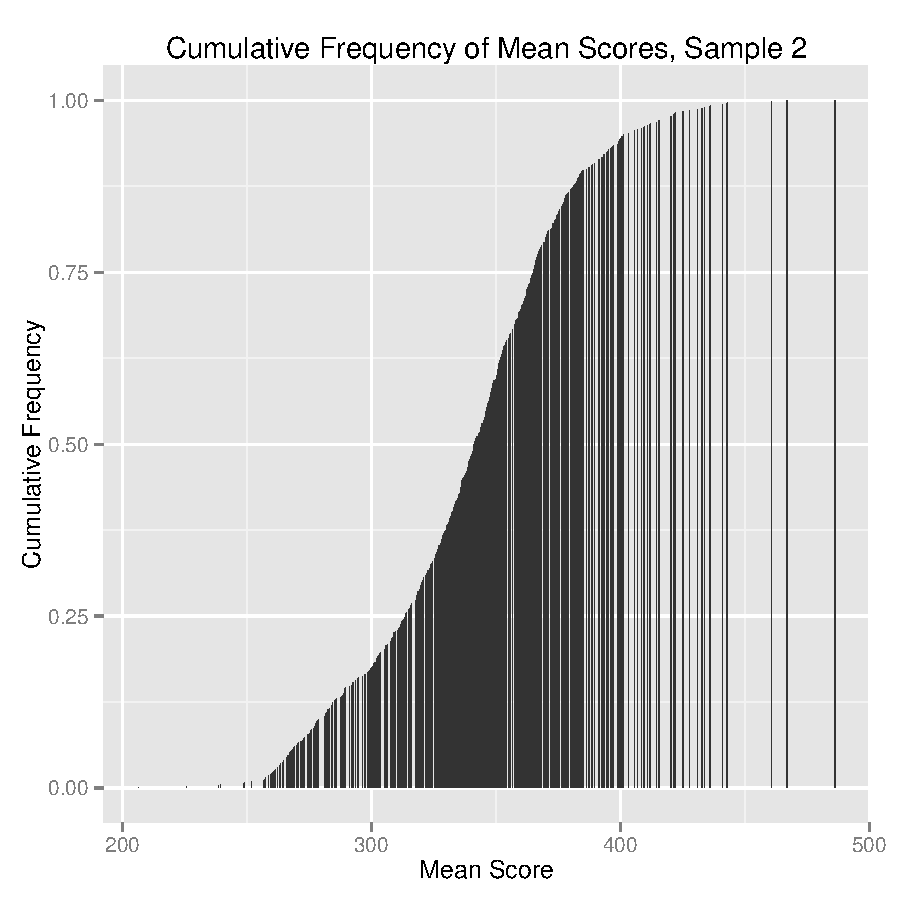
\includegraphics{proj3-fig_scores2}
\caption{Sample Two Score Distribution - Cumulative Frequencies}
\label{fig:Scores_Hist_Two}
\end{centering}
\end{figure}


\begin{figure}[H]
\begin{centering}
\setkeys{Gin}{width=0.5\textwidth}
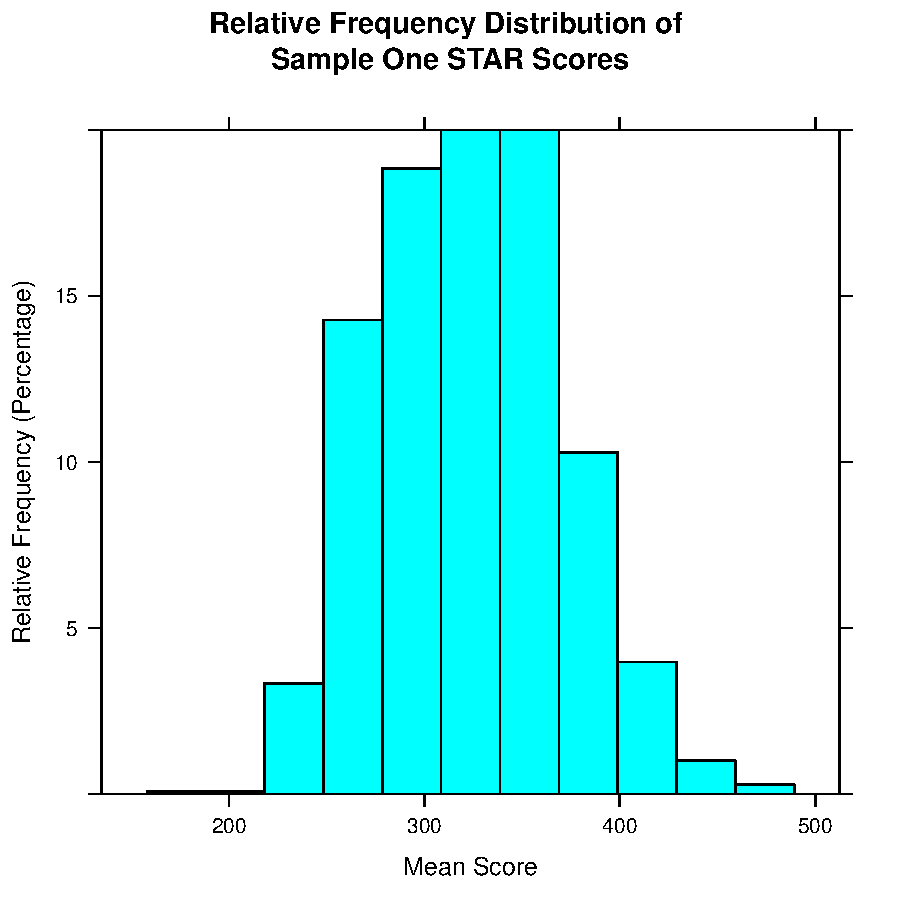
\includegraphics{proj3-rel_freq_scores1}
\caption{Relative Frequencies of the Mean Scores in Sample One}
\label{fig:pie_education}
\end{centering}
\end{figure}


\begin{figure}[H]
\begin{centering}
\setkeys{Gin}{width=0.5\textwidth}
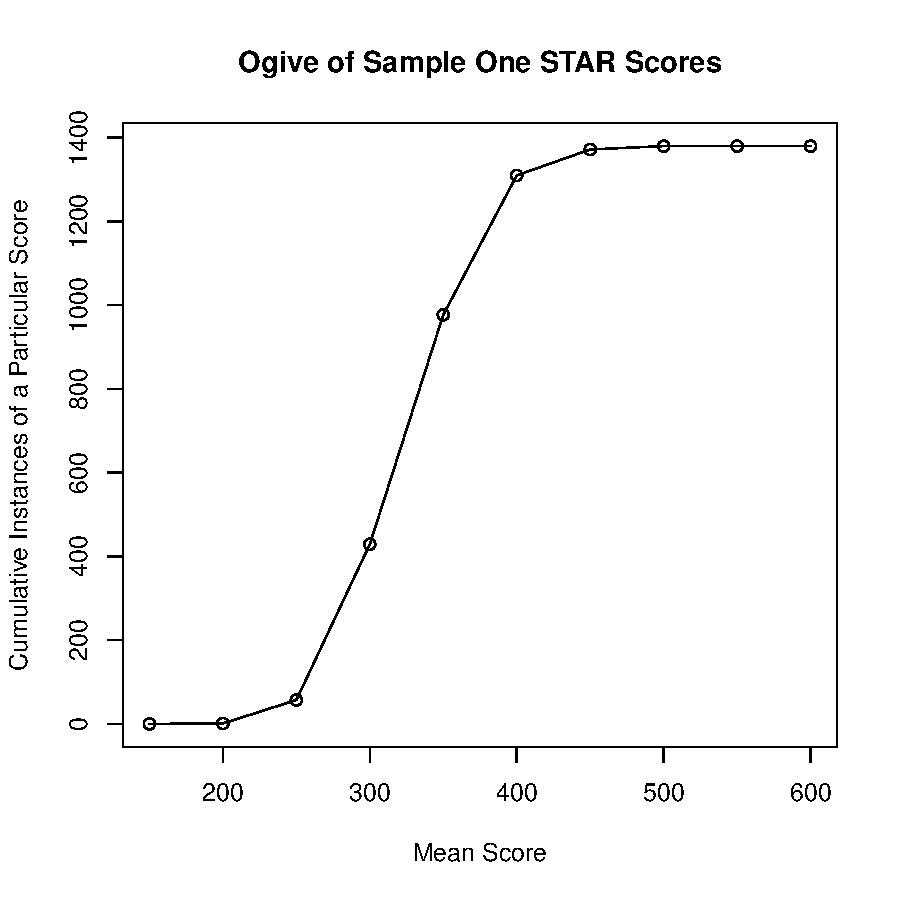
\includegraphics{proj3-ogive}
\caption{Cumulative Frequency Distribution, Sample 1 Scores}
\label{fig:pie_education}
\end{centering}
\end{figure}

\subsection{Summary Statistics}

5 Number Summary of STAR Scores, Sample 1:
\begin{Schunk}
\begin{Soutput}
   Min. 1st Qu.  Median    Mean 3rd Qu.    Max. 
    170     291     325     325     356     477 
\end{Soutput}
\end{Schunk}


5 Number Summary of STAR Scores, Sample 2:
\begin{Schunk}
\begin{Soutput}
   Min. 1st Qu.  Median    Mean 3rd Qu.    Max. 
    226     314     341     339     365     467 
\end{Soutput}
\end{Schunk}

\begin{figure}[H]
\begin{centering}
\setkeys{Gin}{width=0.5\textwidth}
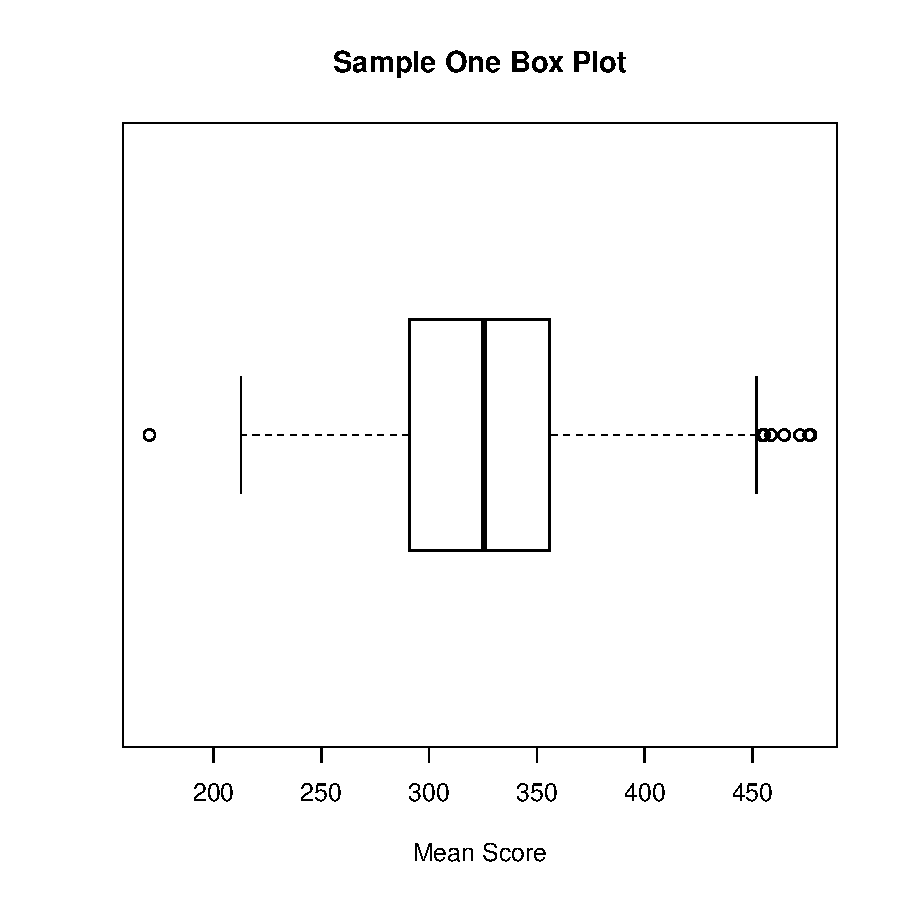
\includegraphics{proj3-bxplot1}
\caption{Modified Box Plot, Sample One}
\label{fig:boxplot1}
\end{centering}
\end{figure}

\begin{figure}[H]
\begin{centering}
\setkeys{Gin}{width=0.5\textwidth}
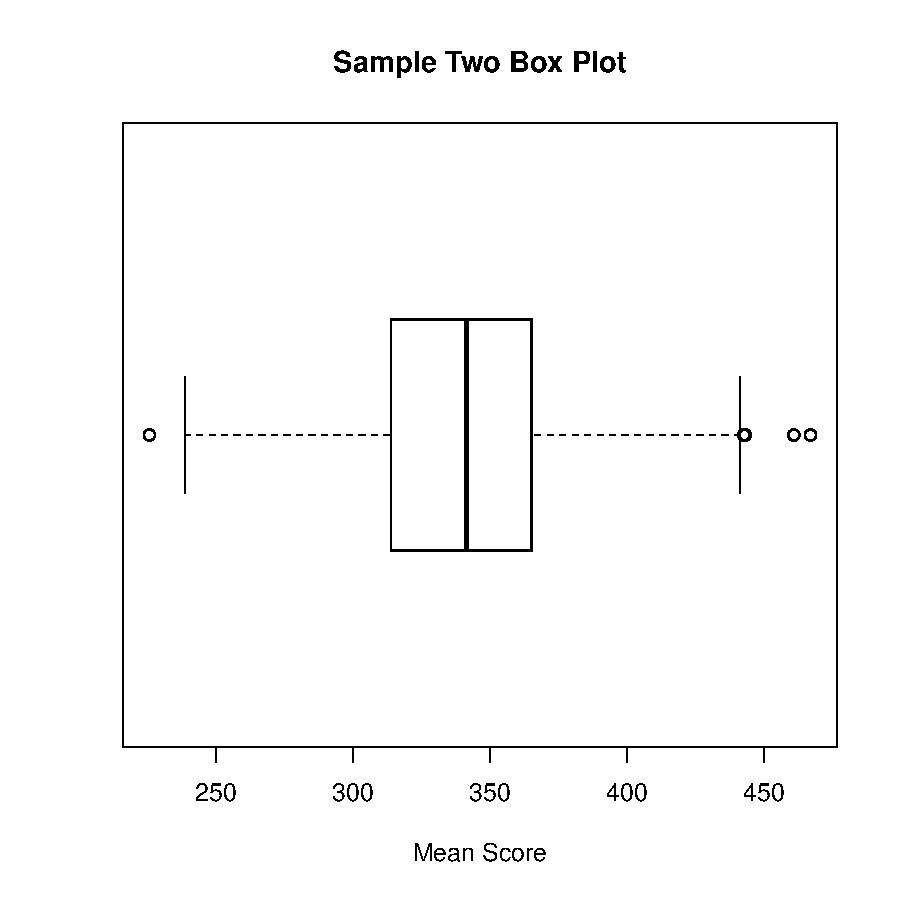
\includegraphics{proj3-boxplot2}
\caption{Modified Box Plot, Sample Two}
\label{fig:boxplot2}
\end{centering}
\end{figure}

\hrulefill

\subsection{Summary Statistics}
Usual Values, Sample 1:
234.05 < 324.746 < 415.442


Usual Values, Sample 2:
258.432 < 338.96 < 419.488


\subsubsection{Confidence Intervals}

Since we the sample means are being examined, we turn to the $t$ test to determine the 95\% confidence intervals for both samples. With 59 degrees of freedom, this yields a critical value $t_{\alpha/2}$ of $\pm 2.000$. 


\textbf{Sample 1:}

$E =$11.709

95\% Confidence Interval: 313.037 < 324.746 < 336.455


\textbf{Sample 2:}

$E =$10.396

95\% Confidence Interval: 328.564 < 338.96 < 349.356

That is, we are 95\% confident that the confidence intervals above contain the true values of $\mu$, the ppopulation mean.

\hrulefill

\subsection{Hypothesis Test}

We test the claim that the two sample means are equal to eachother, or that

\begin{align*}
		H_0: \mu_1 = \mu_2 \\
		H_1: \mu_1 \neq \mu_2,
\end{align*}

where $\mu_1$ and $\mu_2$ are the mean STAR scores of the first and second samples respectively.

To do so, we turn to a $t$-test comparing the means from two indpendent populations for which the population means are not known, which a significance level of .05.

We find that the test statistic is $t =$-1.816. Using technology, the following results are obtained:
\begin{Schunk}
\begin{Sinput}
> t.test(scores1, scores2, var.equal=T, paired=F)
\end{Sinput}
\begin{Soutput}
	Two Sample t-test

data:  scores1 and scores2
t = -6.86, df = 2038, p-value = 8.988e-12
alternative hypothesis: true difference in means is not equal to 0
95 percent confidence interval:
 -18.3 -10.2
sample estimates:
mean of x mean of y 
      325       339 
\end{Soutput}
\end{Schunk}

Because the p-value is much less than the significance level of 0.05, we reject the null hypothesis and conclude that there is sufficient evidence to support the claim that the two populations means are \textit{not} the same.

\section{Conclusion}
The chosen county codes, 39 and 20 for samples 1 and 2 respectively, correspond to San Joaquin and Madera counties. With only slightly over 100 miles between the two counties, there would not be much variation expected, and in fact, looking at the means and medians of both areas, they appear at first glance to have extremely similar scores. However, with such a large sample, the t-test shows that there is evidence to support a small but true difference in the actualy means.

This difference is slightly evident in the analysis from earlier sections as well. For example, examining their quartile ranges shows that while the 75th quartile and maximum scores were very similar, the 25th quartile and minimum scores varied much more.

Interestingly, the cumulative frequency distribution and the ogive for the two sampled scores show sharp increases in the 300-400 range, which according to the 150-600 point scale, puts a large majority of the sampled students very close to a 50\% average on these exams, nearly 10\% less than what many schools classify as failing grades. However, this also suggests that the test scores may be approximately normally distributed.

With the possibility of variance in test scores based on location, and considering the legislative actions that are put into motion based upon schools' performance on these exams, the results of this analysis show that it may be prudent to carefully examine the consistency of curricula across counties and school districts.


%\bibliographystyle{plain}
%\bibliography{physbib}

\end{document}
